\section{Proposed Method}
\label{proposed_method}
% In this Section, we will discuss our complete architecture. But first, we will examine the analysis of different colourspace image representations for the haze removal task. Then we will present the detail about the architecture of the proposed model with an overview of the model. In the end different losses and metrics and their influence on the proposed network will be present.

 \begin{figure*}[ht]
    \centering
    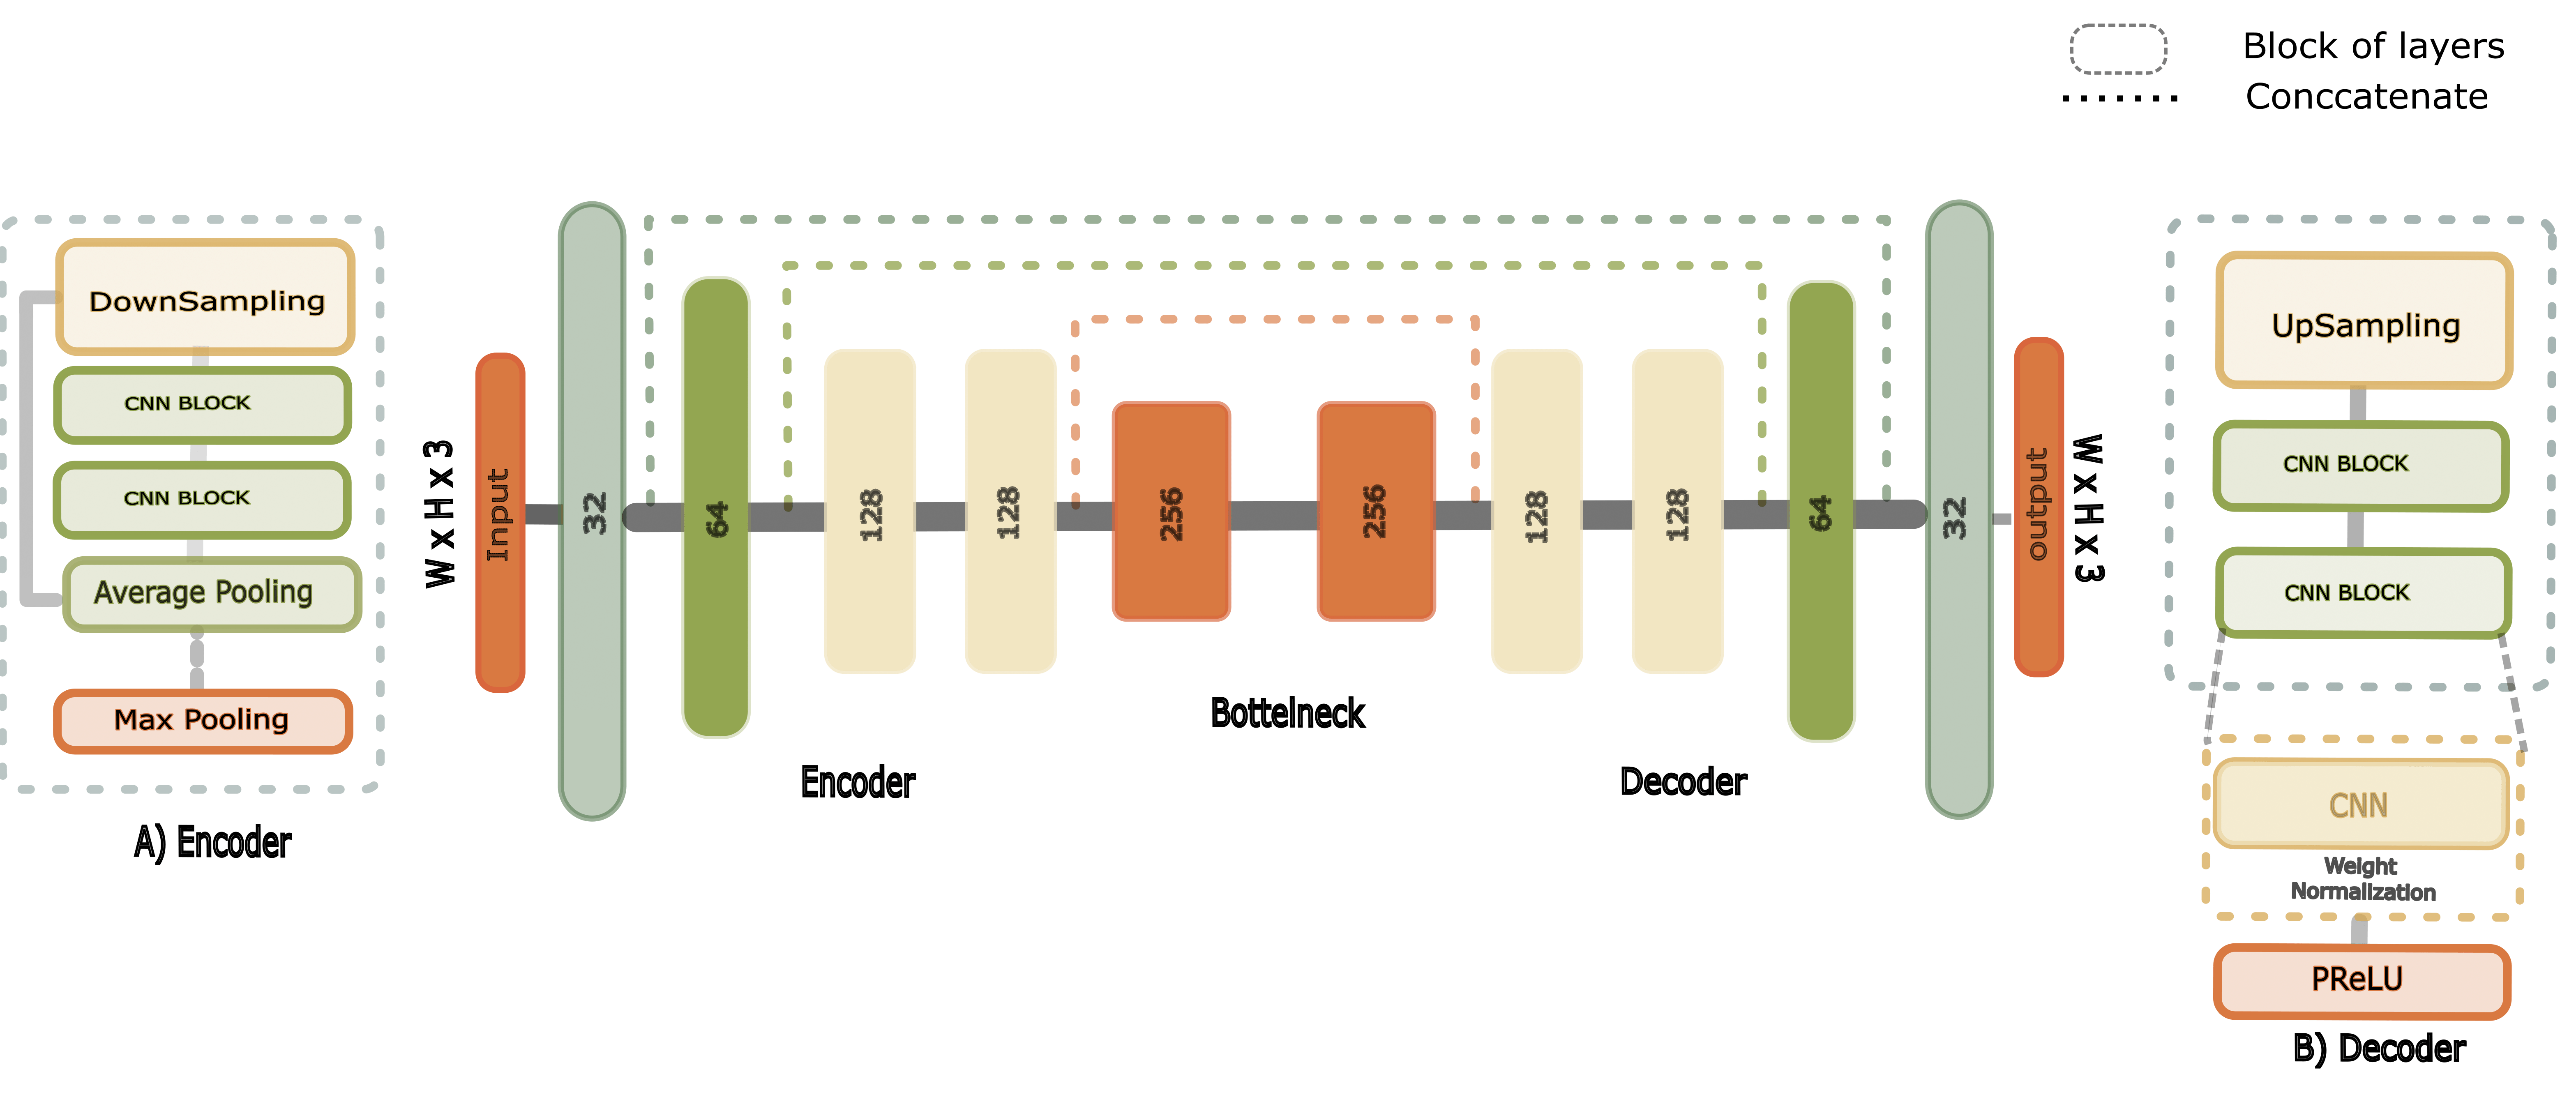
\includegraphics[height=0.5\textwidth, width=0.99\textwidth]{images/i4c_haze.png}
    \caption{The architecture we used in this paper for haze removal. A) Encoder block and B) Decoder block}
    \label{fig:haze_removal_model}
\end{figure*}
\subsection{Colour space}\label{color_space}
We compared RGB and YCbCr colourspace as training inputs to our neural network. We determined that the YCbCr image representation works very well on image haze removal. The YCbCr colourspace is mainly used in image enhancement and image super-resolution tasks because it represents information better than RGB and is noise free compared to RGB colourspace. Recently, YCbCr image representation has shown exceptional outcomes in haze removal tasks. 
As Bianco et al. \cite{hr_haze} showed in their experiment, the mean squared error \textit{(MSE)} \eqref{eqn:mse} is qualitatively better in YCbCr colourspace than RGB because atmospheric illumination in hazy images affects more Y channel more. A better \textit{MSE}  score in YCbCr colourspace is the direct reason for better peak-signal-to-noise ratio \textit{(PSNR)}. Therefore to evaluate the methodology, we will be using YCbCr colourspace as our primary image input representation.
\subsection{Model overview}\label{model_overview}
We prioritise performance, efficiency and simple architecture for our neural network model. The proposed technique is miniature and straightforward to conduct yet achieves better performance than the traditional methodology. We experimented with different approaches that will advance our expectations from our model. The proposed architecture is a U-Net-based formation of encoder, bottleneck and decoder. Each of the sub-formations is a set of cautiously selected blocks of layers that meet close to our prioritise. 
\\
Our end-to-end network's encoder and decoder are composed of convolutional blocks. Each of these blocks contains manually designed layers. Such as the encoder is constructed of downsampling layers and convolutional layers with pre-defined pooling. Whereas the decoder is created using upsampling layers and convolutional layers. These blocks coupled with the skip connection make our network end-to-end. We avoided the batch-normalization layer because of its poor performance on small batches, expensive computation and dissimilarity between training and testing. We used weight normalization because of is computationally inexpensive and gives better weight initialization. We used parametric  PReLU as our activation function since PReLU's learn parameters on how activation should be permitted for negative values.The bottleneck is created with only convolutional layers with fixed weights and biases. 
\subsection{Model architecture}\label{model_arch}
As outlined in Fig \eqref{fig:haze_removal_model}, the encoder is stacked with multiple convolutional blocks. Each of these blocks contains a set of convolutional layers, average pooling, max pooling, weight normalization and parametric ReLU. We downsampled the input by half i.e. the stride of two and raise the weight by a factor of two. The feature extracted in the block passed to the next block till they reach the bottleneck. The encoder is directly connected to the decoder via skip connection. Such that, the initially learned parameter could directly transfer to the decoder. The bottleneck is the only phase without any skip connection and sampling.  The input and output size of this phase is equal and the weight is the same for each block. 
\\
The decoder is composed of downsampling convolutional blocks. The decoder has the same set of layers as the encoder except for the downsampling layers such as average pooling and max pooling decoder has an upsampling layer. we used stride two with decreasing weight by a factor of two. For upsampling, we used bilinear interpolation. The decoder is directly connected to encode via skip connections from which the decoder gets learned parameters from an encoder.


\begin{figure*}[ht]
\caption{The results on datasets O-Haze \cite{o_haze} and I-Haze \cite{i_haze}}
\centering
\begin{tabular}{ccc}
Ground-truth  & \multicolumn{1}{c}{Input} & \multicolumn{1}{c}{ Our } \\
 \subfloat[]{\label{set5-original}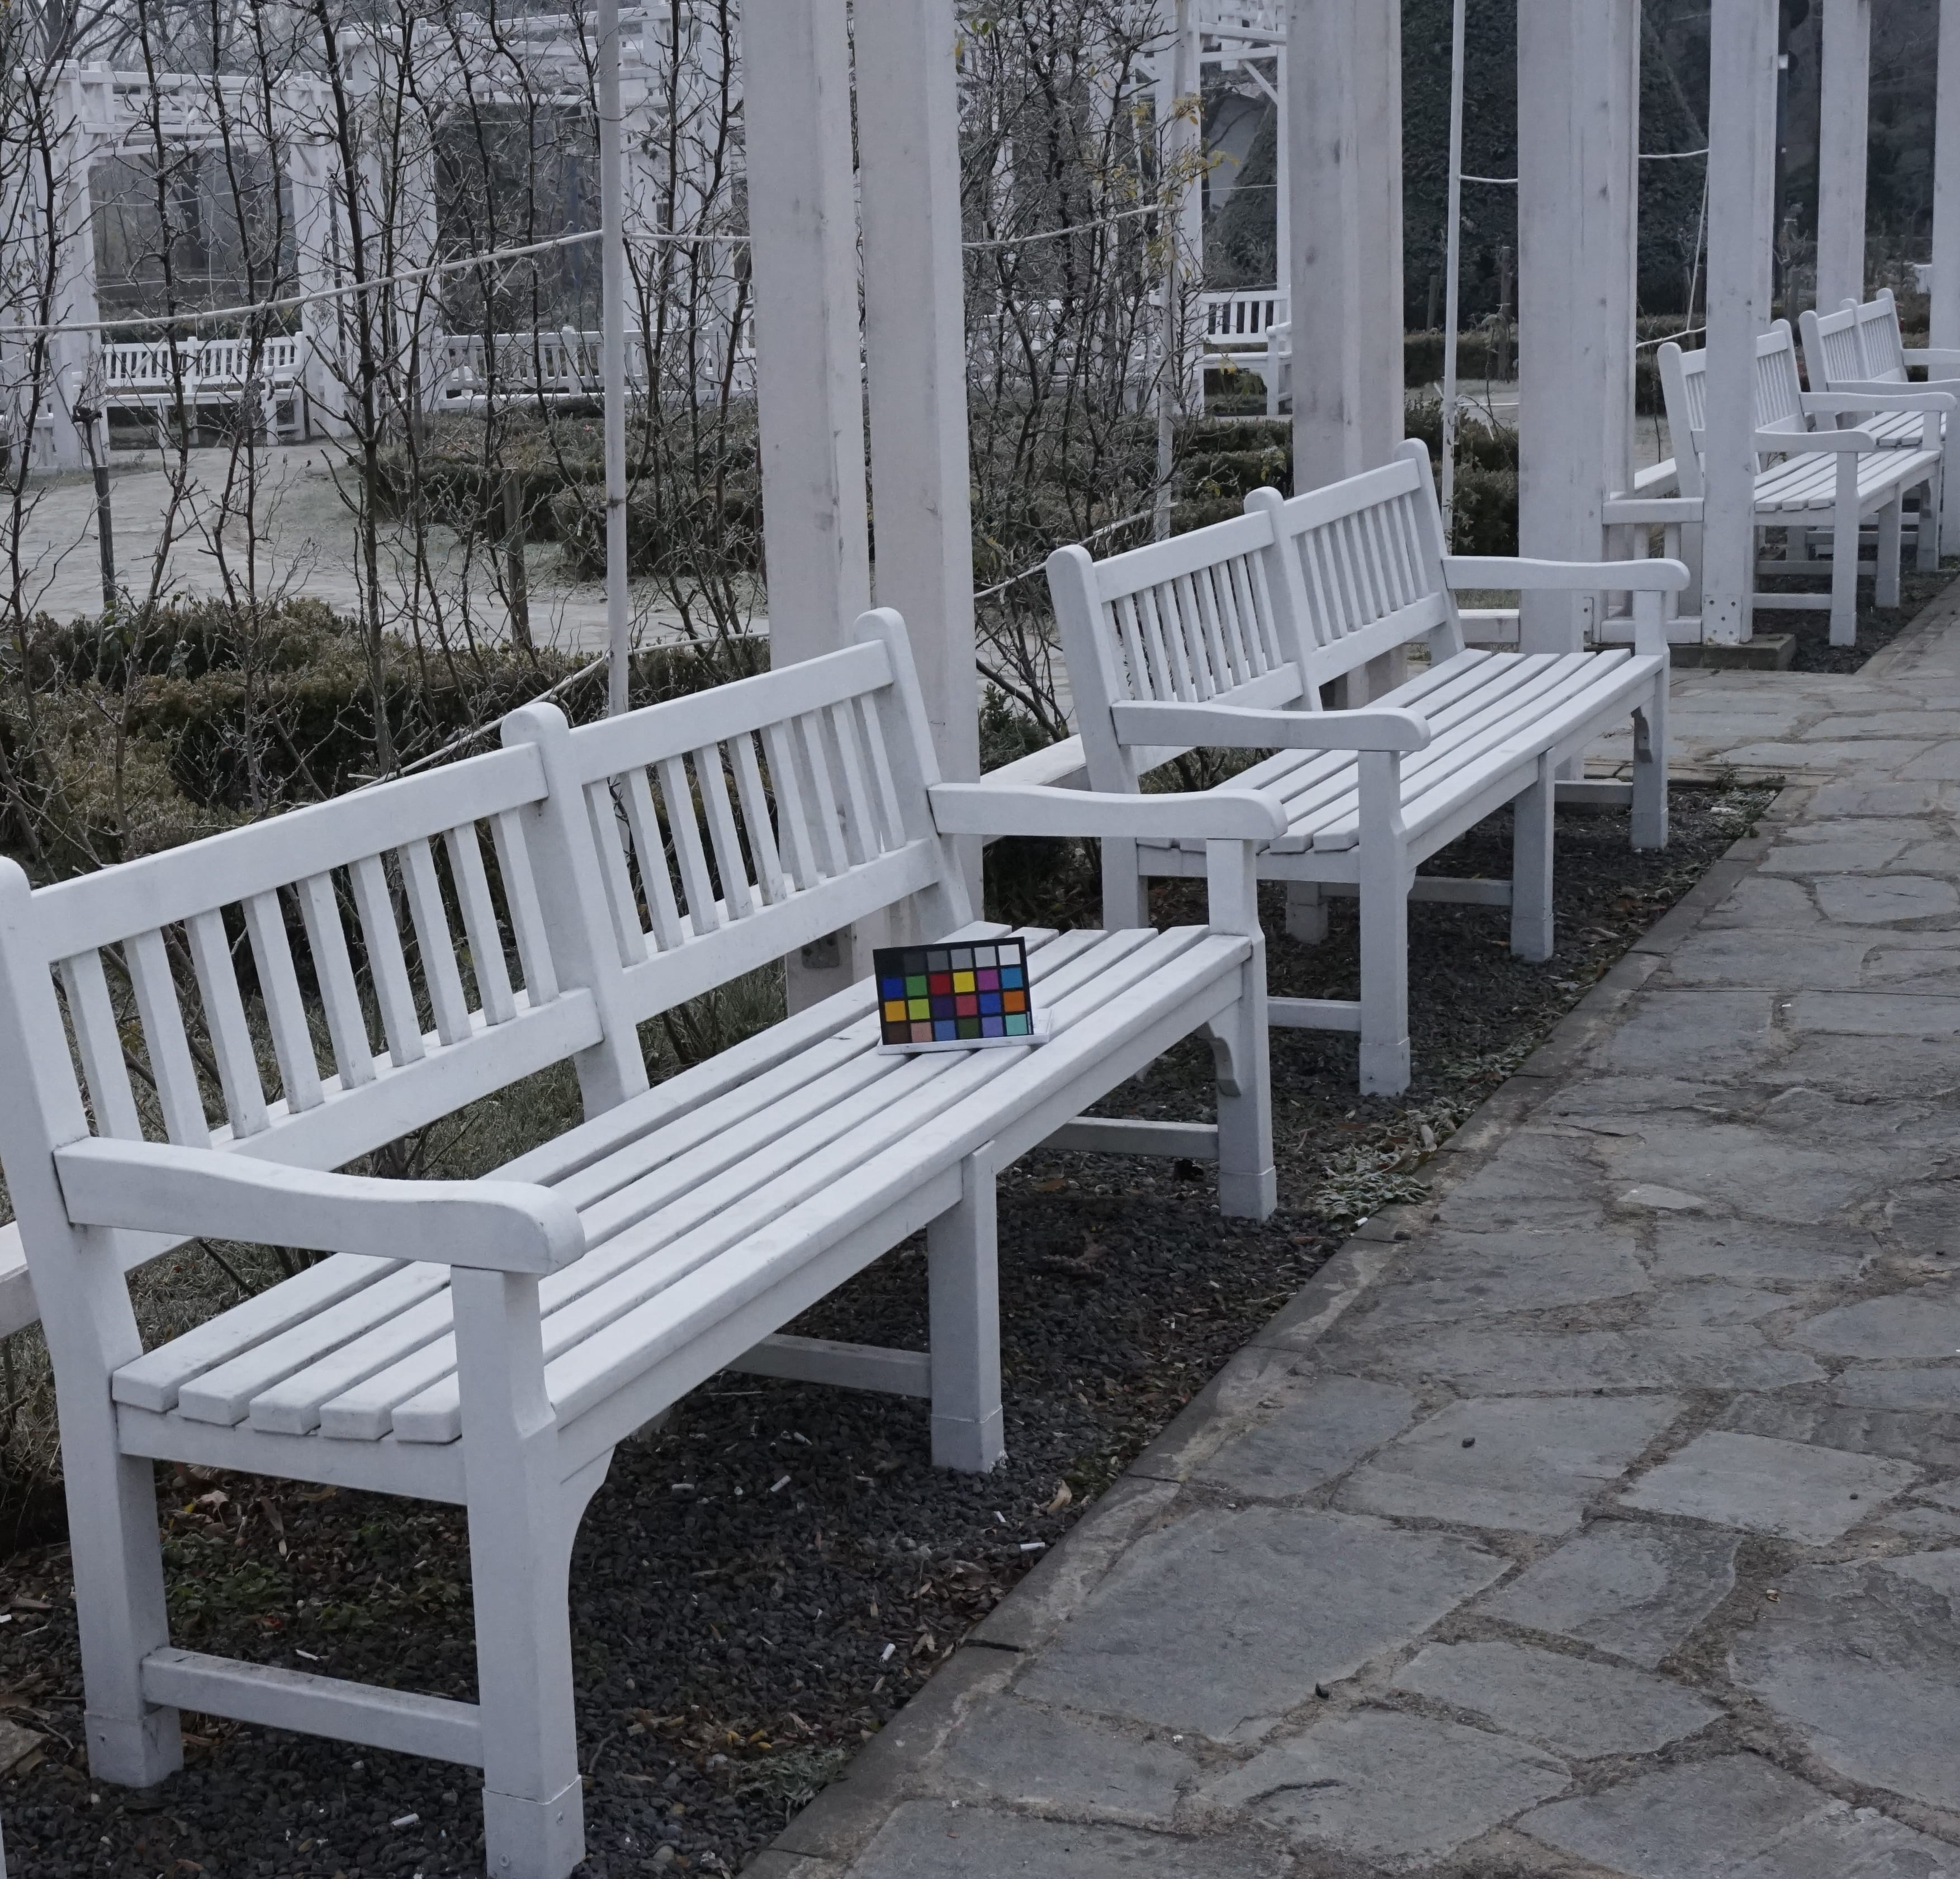
\includegraphics[height=4.2cm, width=4.2cm]{images/40_outdoor_GT.jpg}}  & 
 \subfloat[]{\label{set5-bic} 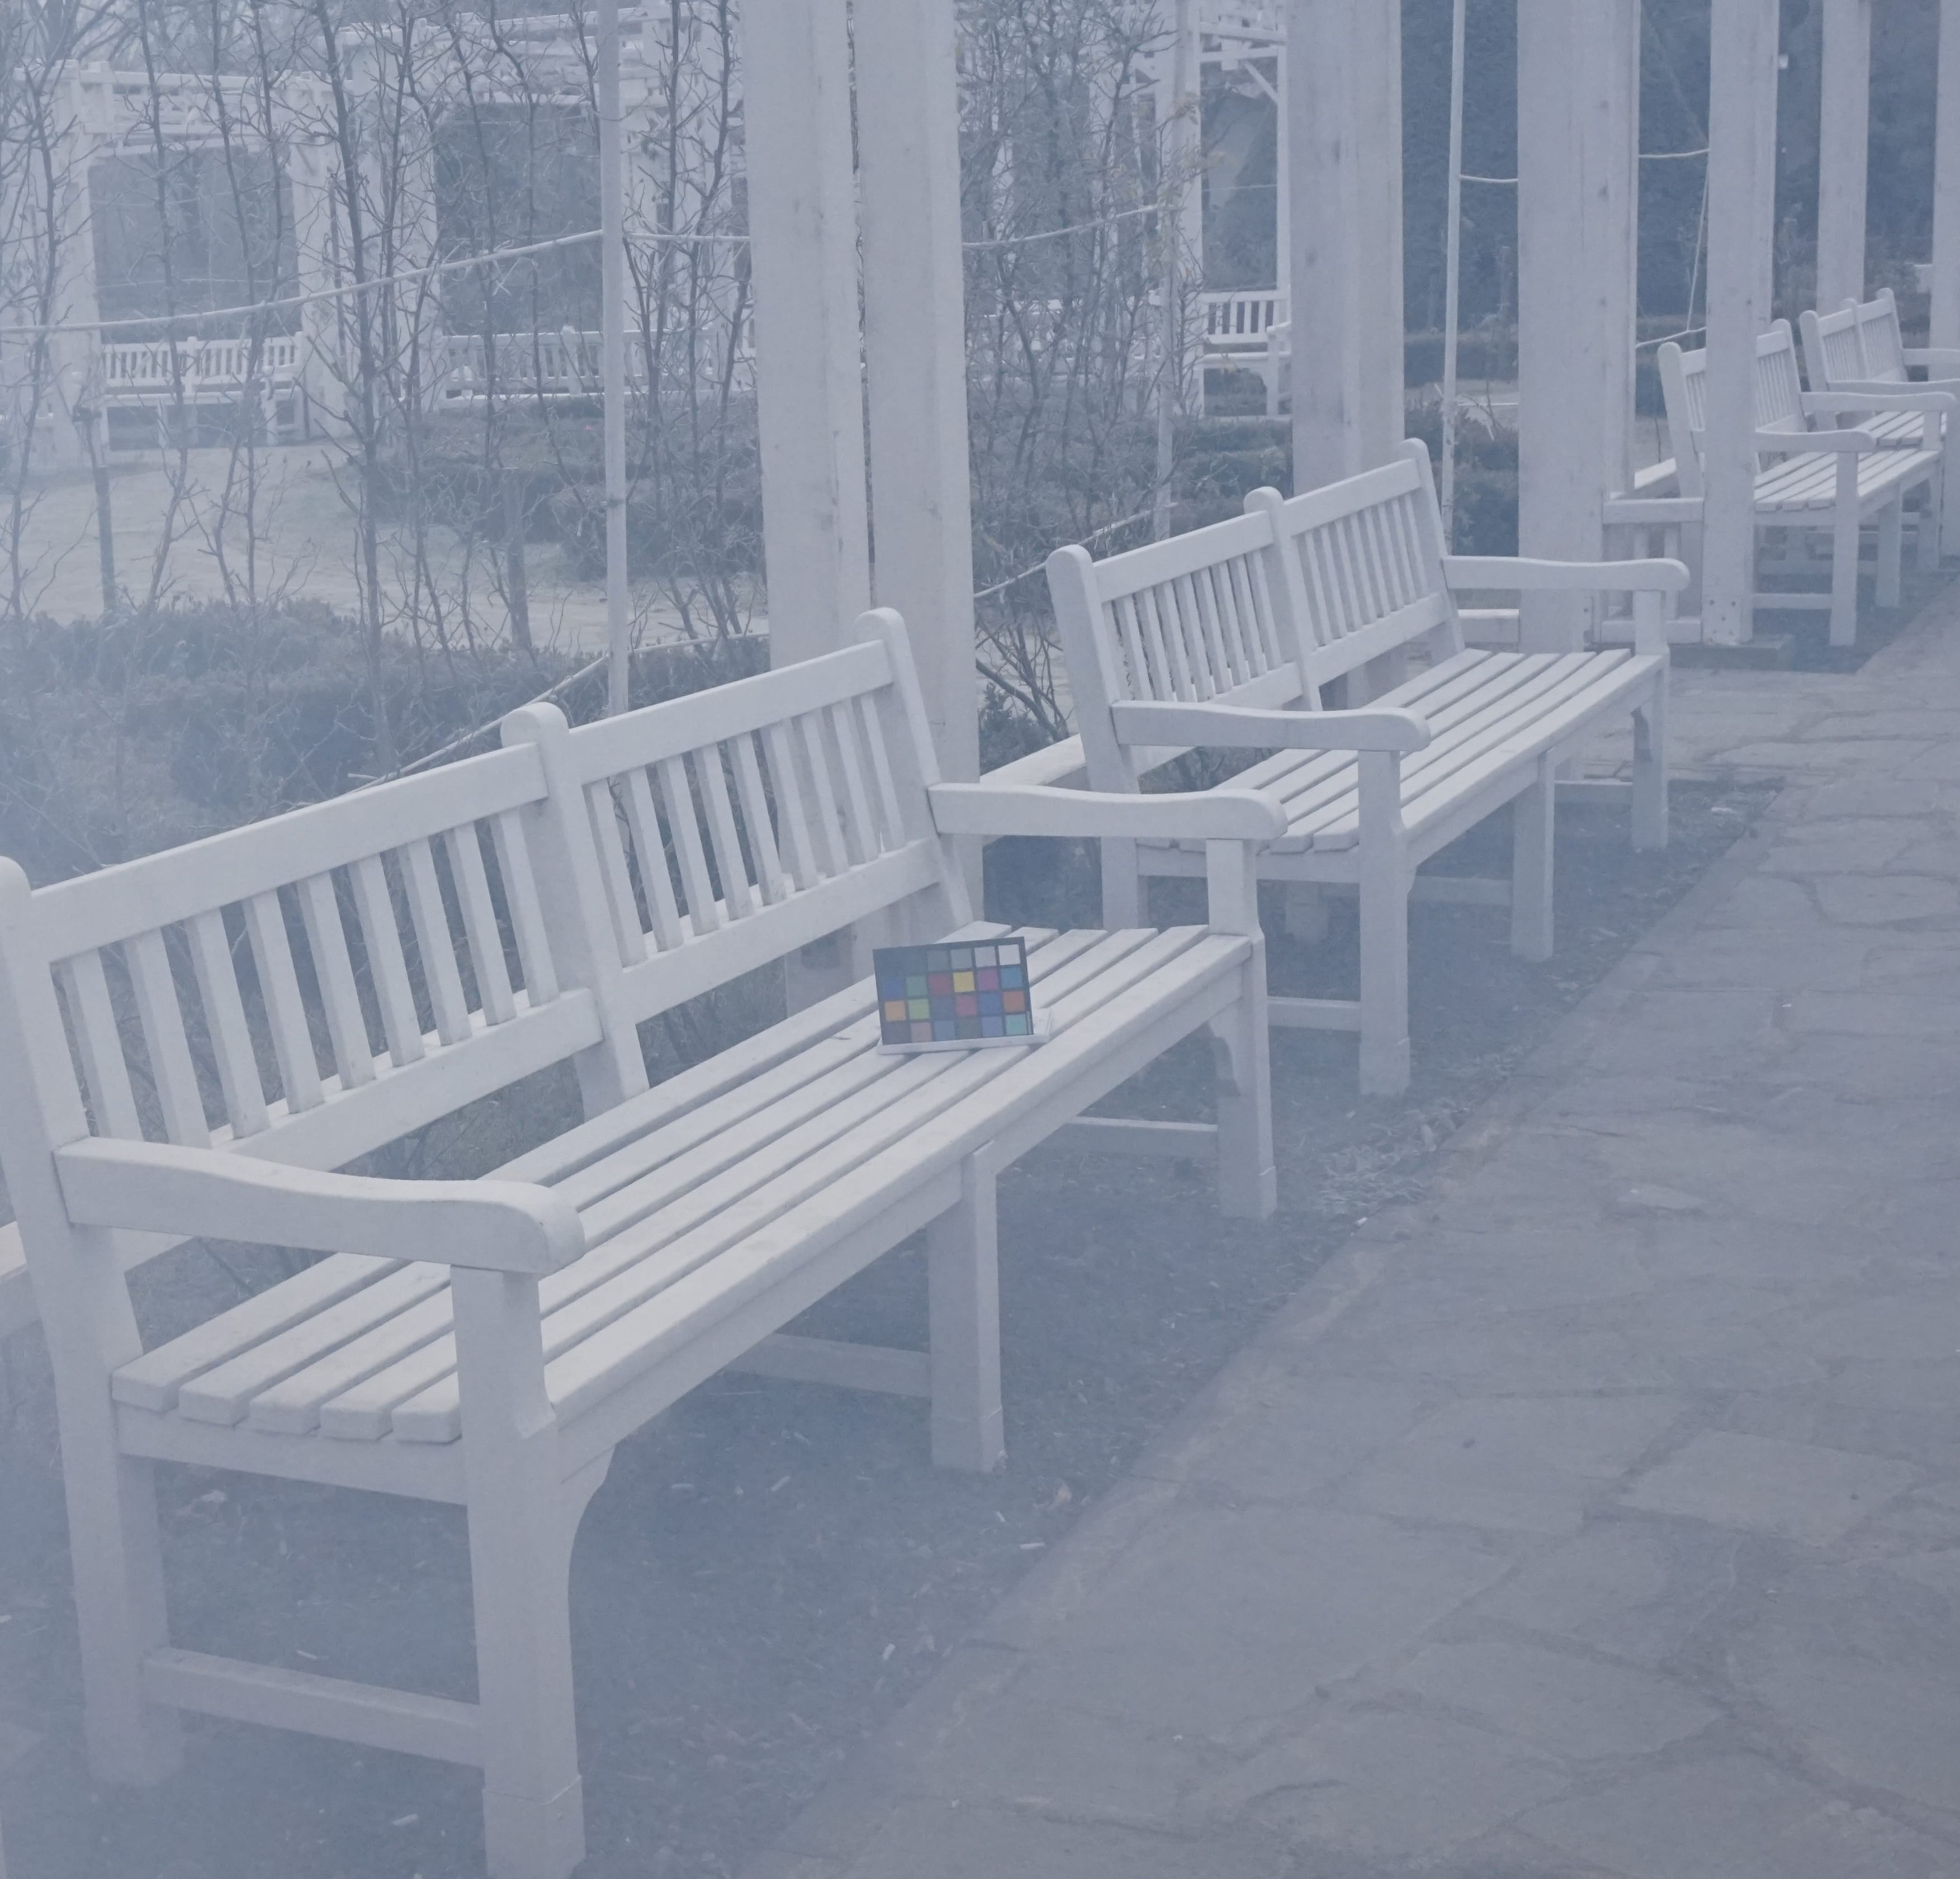
\includegraphics[height=4.2cm, width=4.2cm]{images/40_outdoor_hazy.jpg}} & 
  \subfloat[]{\label{set5-pred}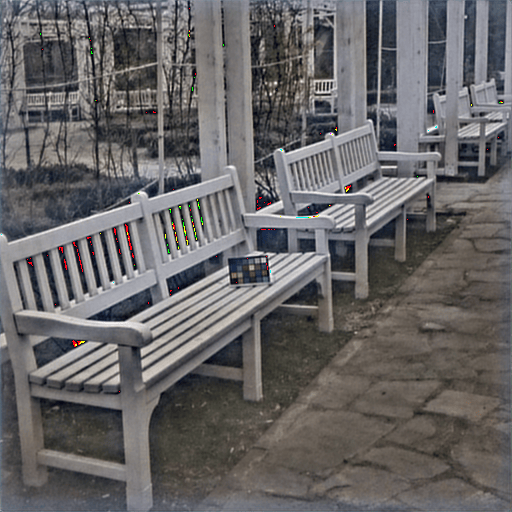
\includegraphics[height=4.2cm, width=4.2cm]{images/O-Dataset_40.png}} \\
 % \subfloat[]{\label{set14-or}\includegraphics[height=4.2cm, width=4.2cm]{images/GT22_dense.jpg}} & 
 %  \subfloat[] {\label{set14-bic}\includegraphics[height=4.2cm, width=4.2cm]{images/22_hazy.png}} & 
 %   \subfloat[]{\label{set14-pred}\includegraphics[height=4.2cm, width=4.2cm]{images/dense22.png}} \\
 \subfloat[] {\label{set14-org}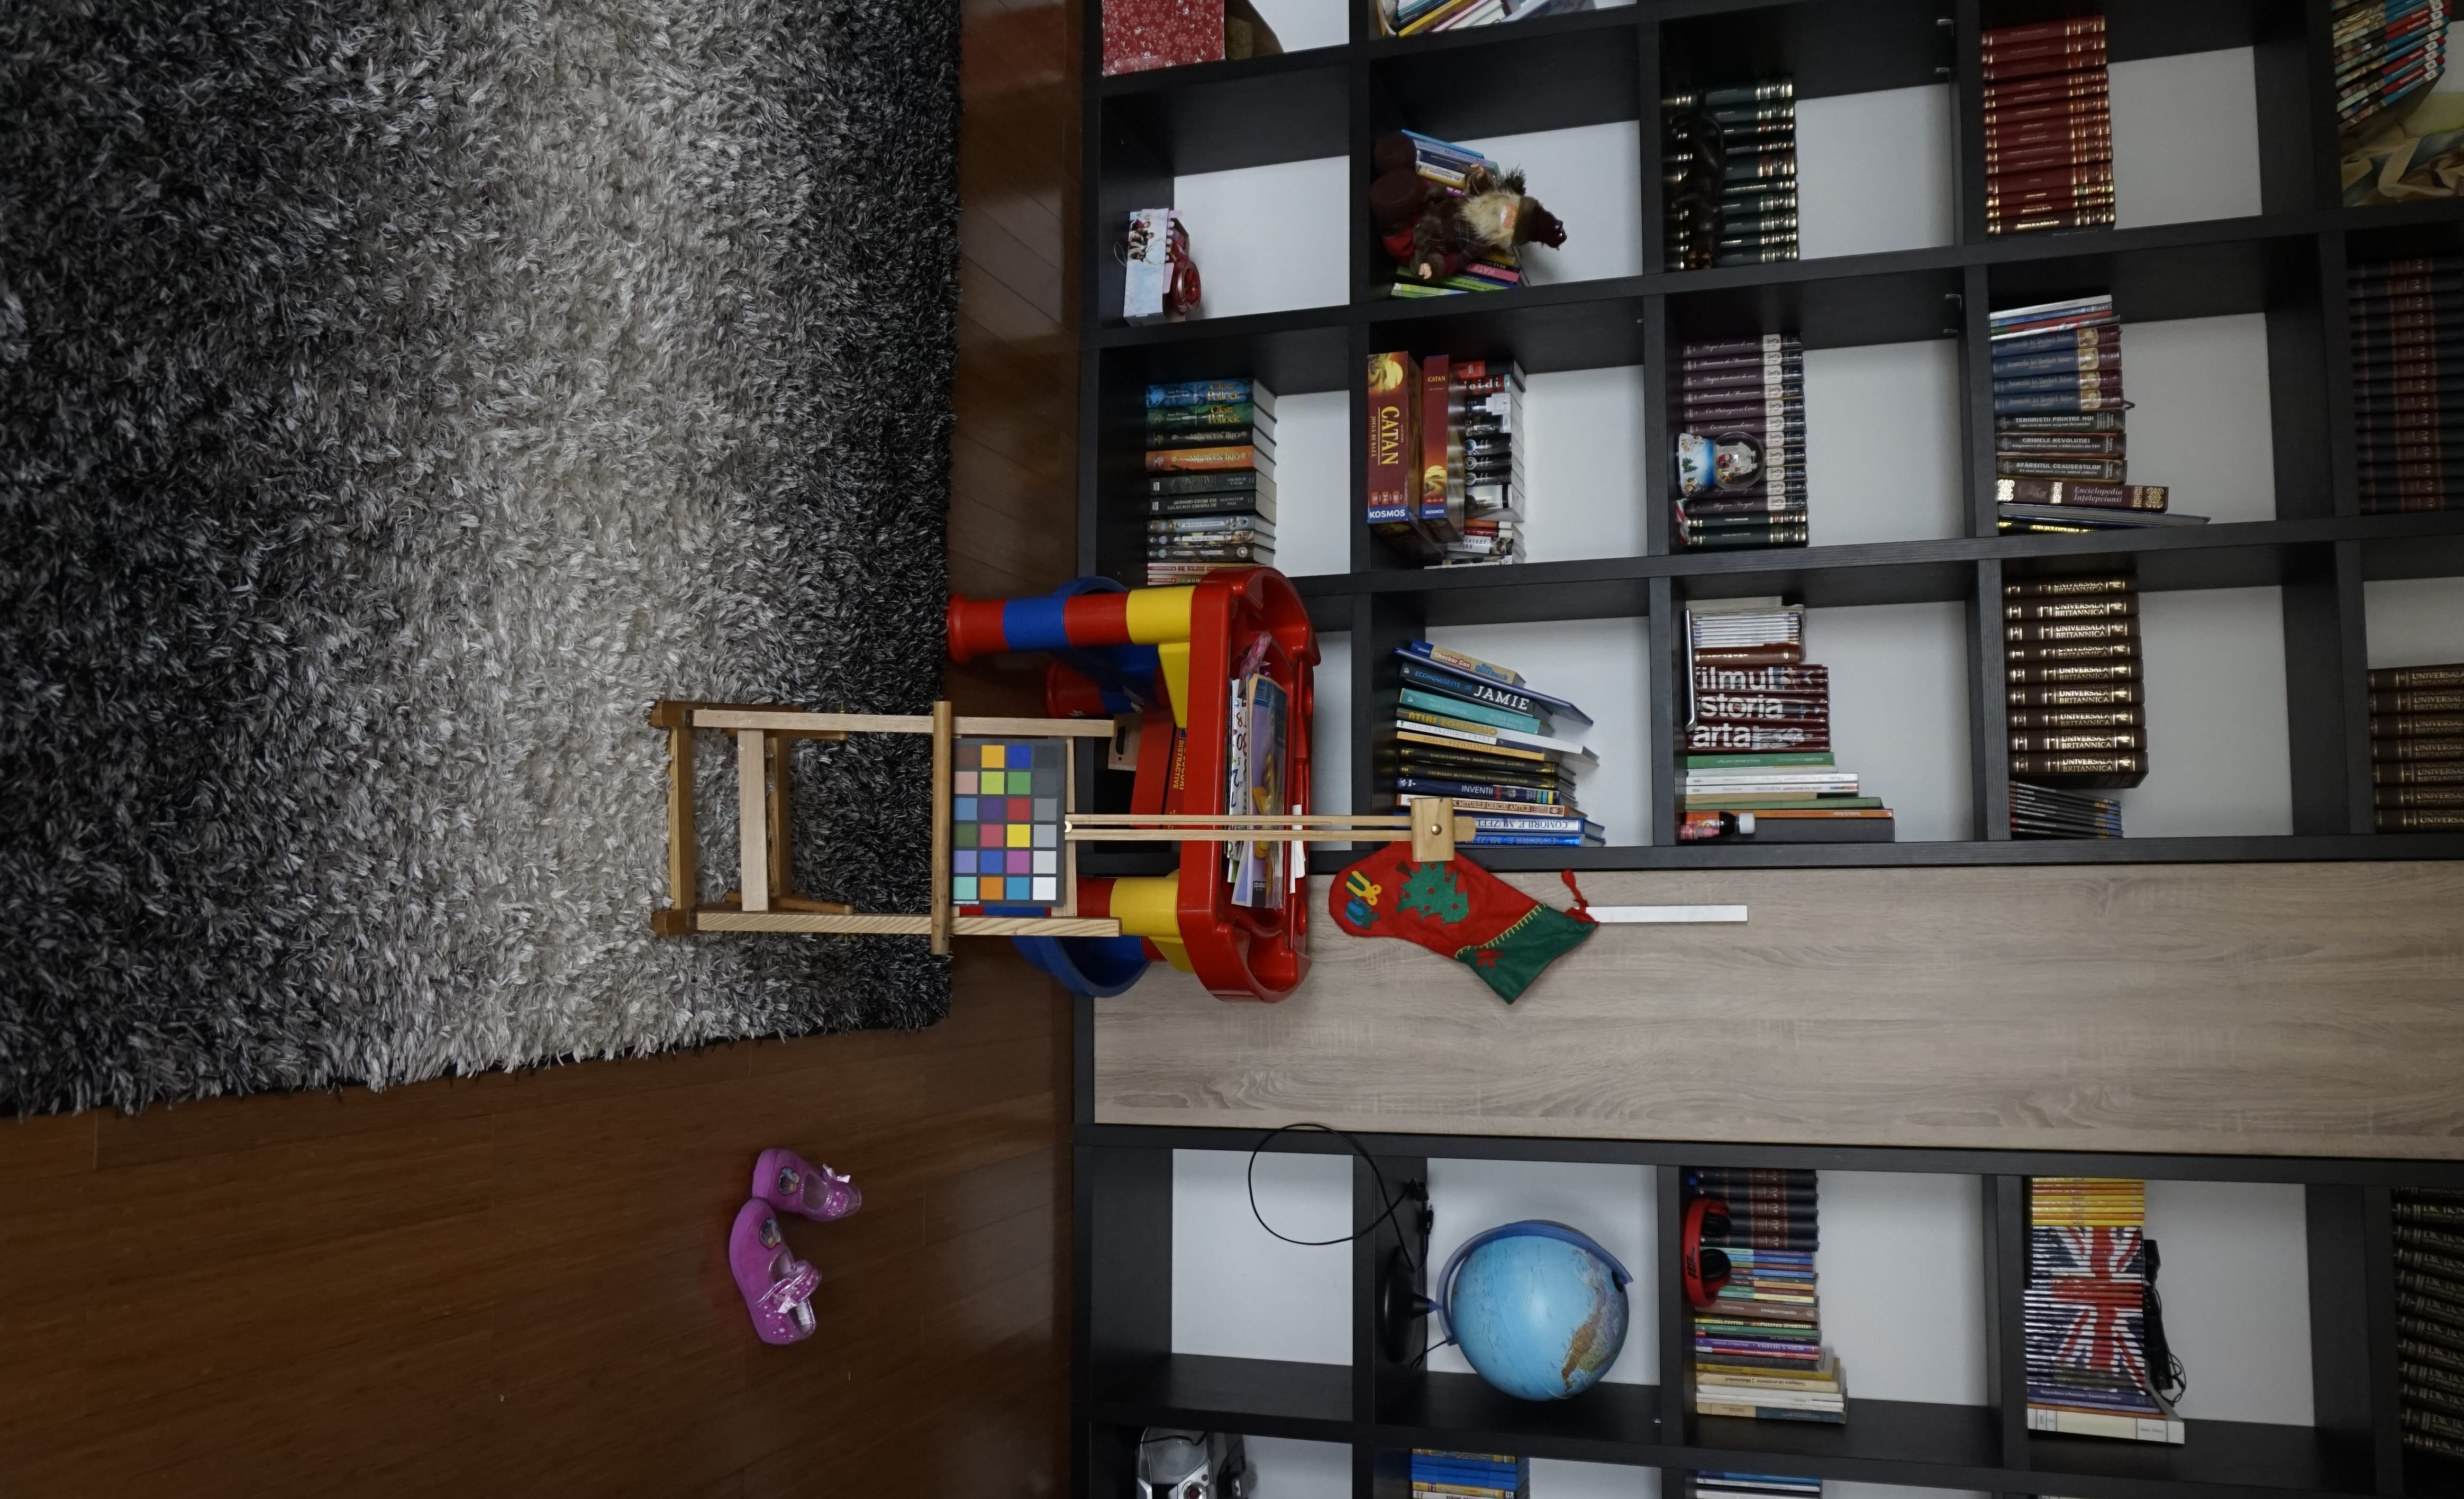
\includegraphics[height=4.2cm, width=4.2cm]{images/02_indoor_GT.jpg}} & 
 \subfloat[]{\label{set14-bicu} 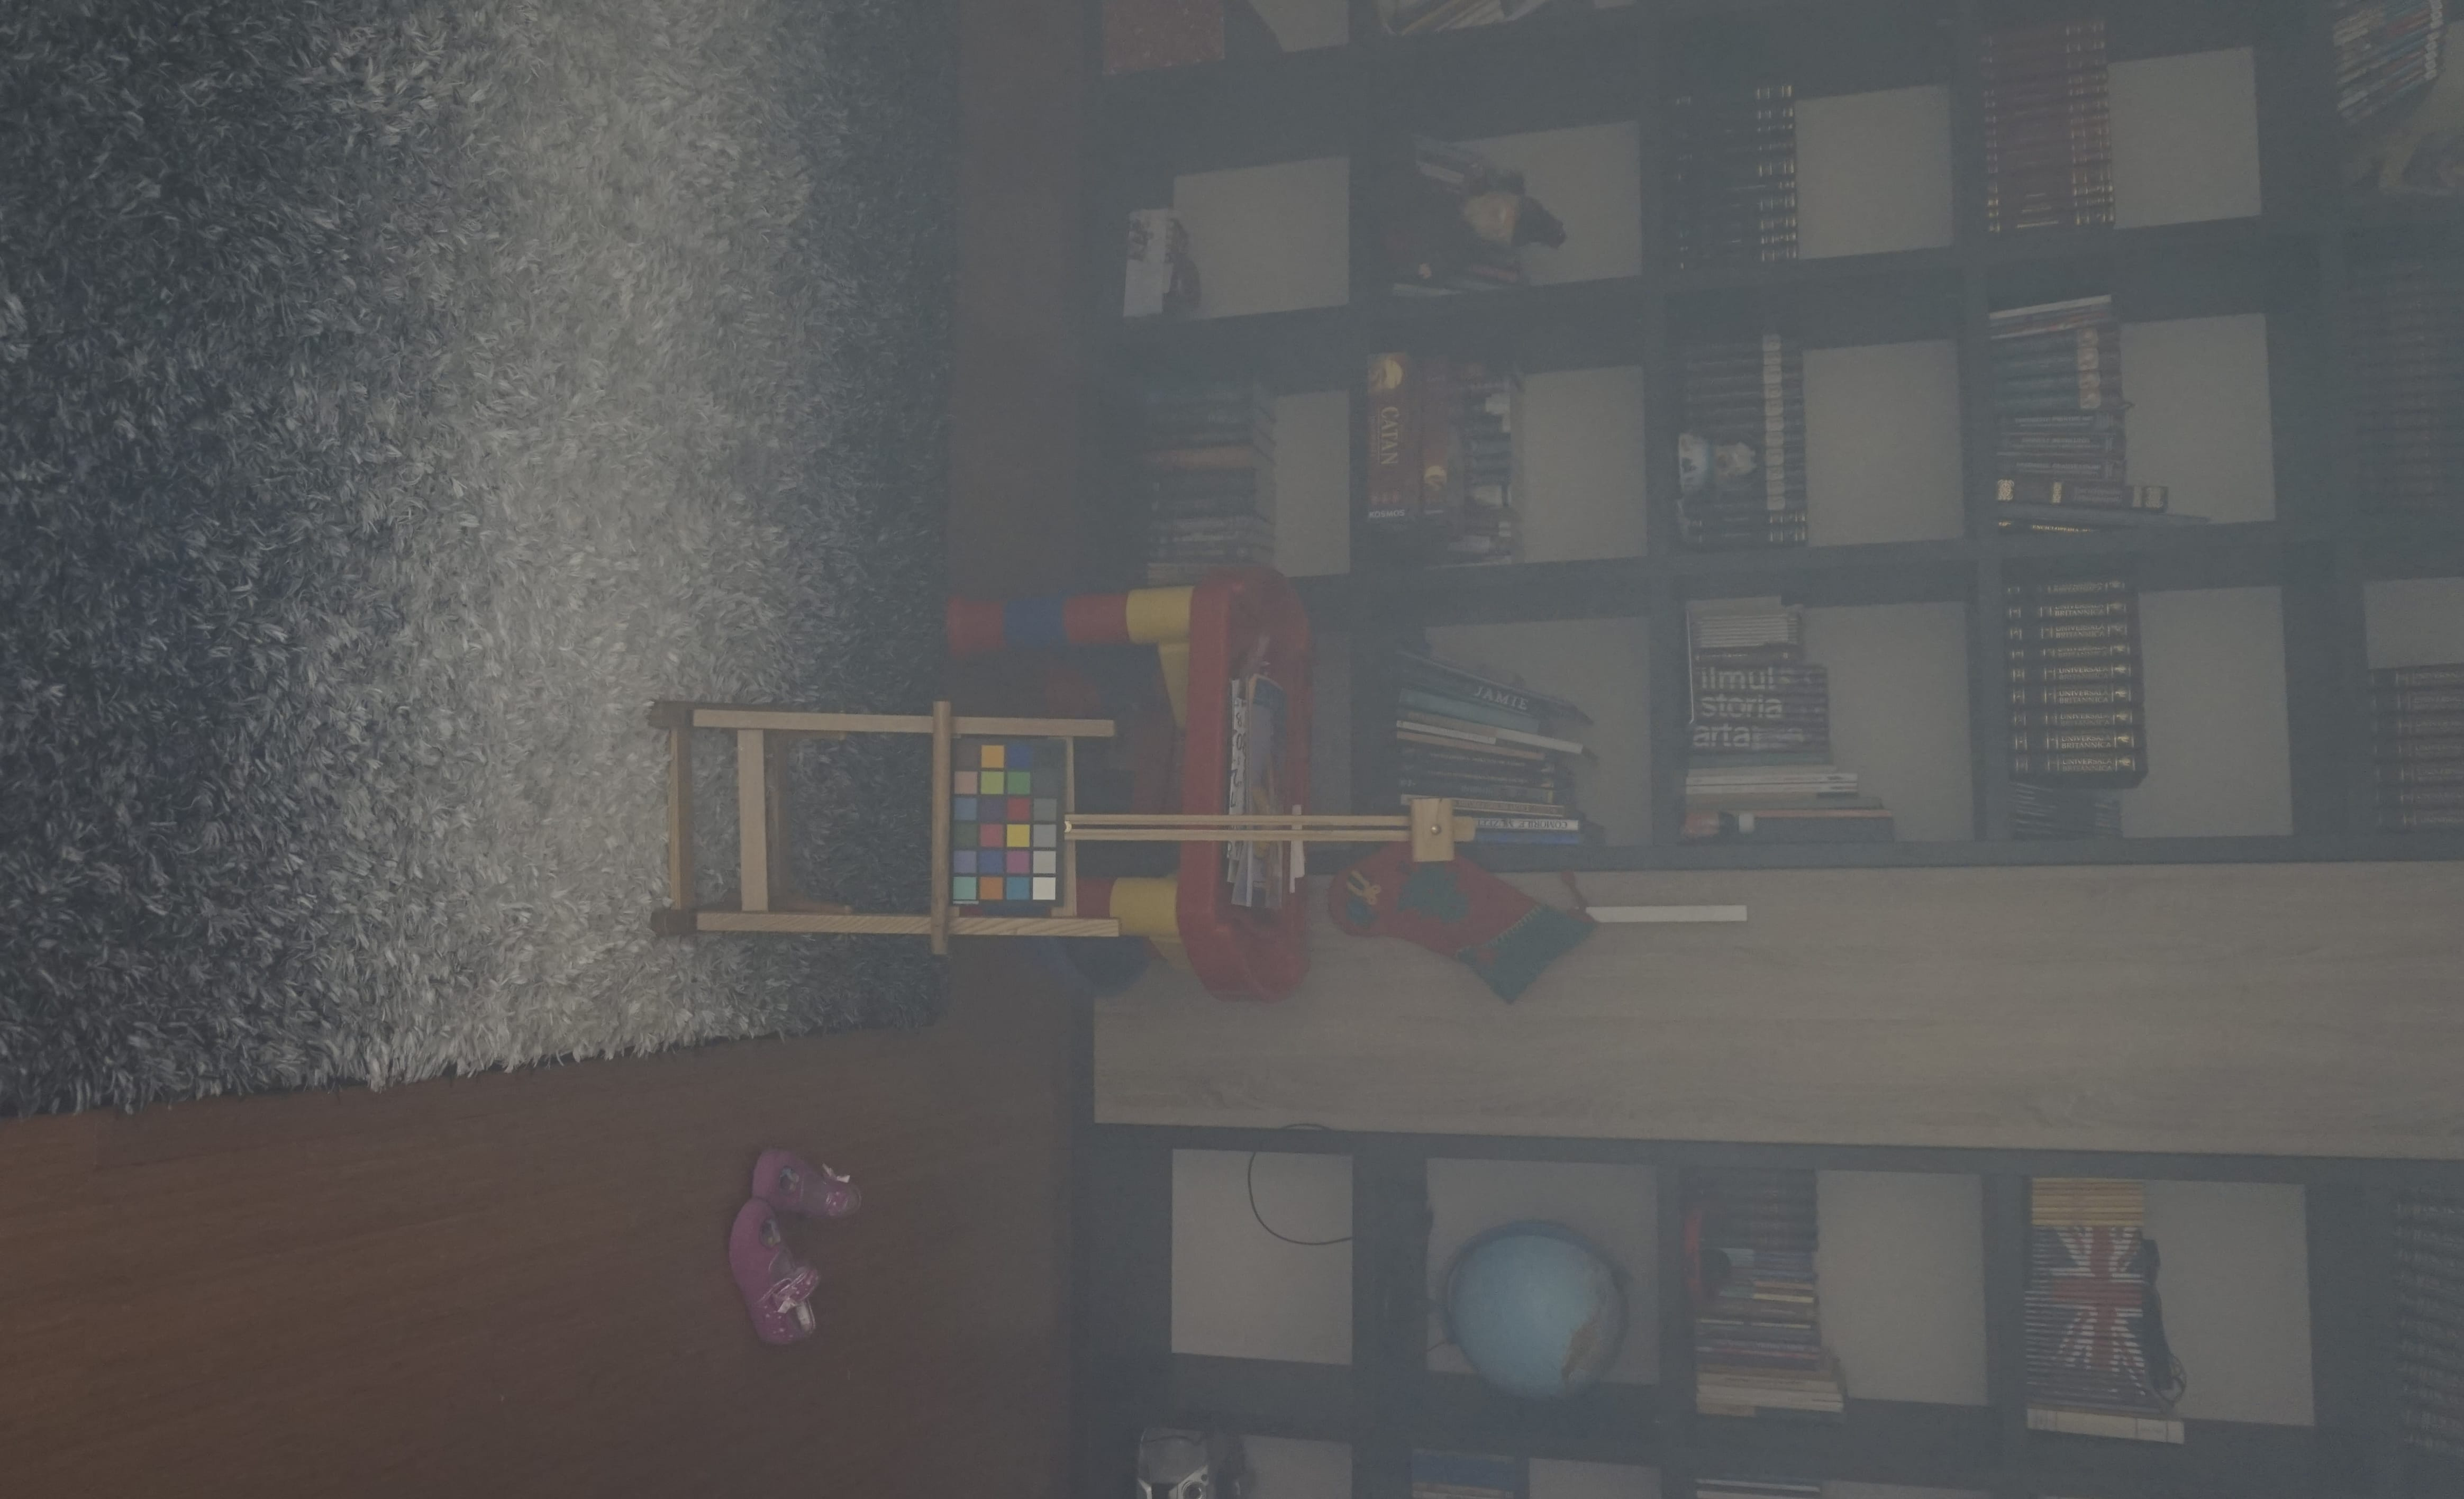
\includegraphics[height=4.2cm, width=4.2cm]{images/03_indoor_hazy.jpg}} & 
 \subfloat[]{\label{set14-predi} 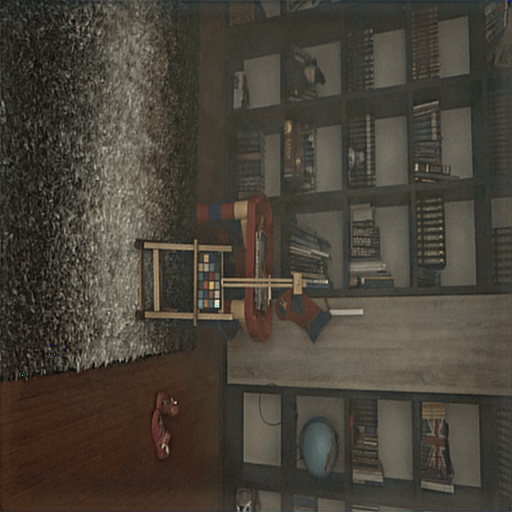
\includegraphics[height=4.2cm, width=4.2cm]{images/I-Dataset_2.png}} 

\end{tabular}
\label{tab:Results}
\end{figure*}

\subsection{Losses and metrics}\label{loss_metric}

The loss function associated with the trained model is stated as follows:
\begin{equation}
\mathcal{L} \ = \ \mathcal{L}_{{1, 2}} \ + \ \mathcal{L}_{FFT} \ + \ \mathcal{L}_{SSIM}
    \label{eqn:total_loss}
\end{equation}
\begin{itemize}
    \item Frequency-domain loss \cite{fft} ($\mathcal{L}_{FFT}$) transforms output images into frequency signals. To increase sharpness and
reduced noise and other artifacts. Let $m$, $n$ dimension of images $I_1$ and $I_2$ , where $K$ is
scaling factor
\textit{FFT} stands for \textit{Fast Fourier Transform} of Image $I$. The Fast Fourier transform is
\begin{equation}
    \mathcal{L}_{FFT} = \mathcal{L}^{\frac{m}{k}\times\frac{n}{k}} =  \frac{k^2}{m \times n} \left | FFT(I_1) - FFT(I_2) \right |^{\frac{m}{k}\times\frac{n}{k}}
    \label{eqn:fft}
\end{equation}
fast algorithm to compute $DFT$ i.e. \textit{Discrete Fourier Transform}. By transforming
images into frequency, we can learn to see the differences in higher dimensional region.
By transforming image signals into a frequency domain for Fourier transform such
that we can enhance the higher frequencies while keeping lower frequencies which will
sharpen the images. 
    \item Smooth $\mathcal{L}_{1}$ loss ($\mathcal{L}_{1}$) is amalgamation of $\mathcal{L}_{1}$ and $\mathcal{L}_{2}$ losses, when the respective 
absolute error is high it behaves like $\mathcal{L}_{1}$ and when the absolute error is close to zero it
behaves like an $\mathcal{L}_{2}$. We used Huber loss \cite{huber} as smooth $\mathcal{L}_{1}$ loss because of its similarity
\begin{equation}
    \mathcal{L}_{\delta}\left ( {a} \right ) \ = \ \left\{\begin{matrix}
{\frac{a^2}{2}} & for \ \left | a \right | \leq  \delta \\ \\
\delta \left ( \left | a \right |- \frac{\delta}{2} \right ) &  otherwise
\end{matrix}\right.
    \label{eqn:l1_loss}
\end{equation}
    \item Mean Square Error (\textit{MSE}) is used as $\mathcal{L}_{2}$ loss function as follows: \\
    
    \begin{equation}
    \mathcal{L}_{2}= \ MSE = \frac{1}{mn} \sum_{1}^{m} \sum_{1}^{n} \left \| \widehat I(n, m) - I^{*}(n, m)  \right \|^{2} 
     \label{eqn:mse}
\end{equation}
Where, $\widehat I$ is predicted image and $I^{*}$ is ground-truth image. 
    \item PSNR is used as a metric for image quality. The higher value indicates better quality. The unit of \textit{PSNR} is \texttt{dB}. We calcuate the \textit{PSNR} as following equation.
    \begin{equation}
    PSNR = 20 \log_{10} \left ( \frac{MAX_{ \widehat I}}{\sqrt{MSE}} \right )
    \label{eqn:psnr}
    \end{equation}
    Where, $\widehat I$ is predicted image based on \textit{MSE}  \eqref{eqn:mse}.
    \item Structural Similarity (\textit{SSIM}) is used as a metric to improve the structural accuracy of predicted output.
    \begin{equation}
        SSIM(x, y) \ = \ \frac{\left ( 2\mu_{x}\mu_{y} \ + \ C_{1} \right) \left ( 2\sigma_{xy} + \ C_{2} \right)}{\left ( \mu_{x}^{2} \ + \ \mu_{y}^{2} + C_{1} \right ) \left ( \sigma_{x}^{2} \ + \ \sigma_{y}^{2} + C_{2} \right )}
        \label{eqn:ssim}
    \end{equation}
     whereas, $\mu _{x}$ the pixel sample mean of x , $\mu _{y}$ the pixel sample mean of y, $\sigma _{x}^{2}$ and the change in variance of x, $\sigma _{y}^{2}$ can effect the variance of y, $\sigma_{xy}$ which is associated with the covariance of x,
     \item Structural Similarity loss ($\mathcal{L}_{SSIM}$) is used retain structural similarity of reconstructed image we minimized \textit{SSIM} loss. The loss function is stated as below,
     \begin{equation}
         \mathcal{L}_{SSIM} = \frac{\left ( 1- SSIM \right )}{2}
         \label{eqn:ssim_loss}
     \end{equation}
     where as \textit{SSIM} is from \eqref{eqn:ssim}
\end{itemize}


% Please add the following required packages to your document preamble:
% \usepackage{graphicx}
\begin{table}[h]
\caption{The quantitative  result of different traditional methods with our model on I-Haze, O-Haze.
}
\label{tab:my-table}
% \resizebox{\columnwidth}{!}{%
\begin{tabular}{cccccc}
\multicolumn{6}{c}{\textit{\textbf{I-Haze}}  \cite{i_haze} }                                   \\ \hline
\textbf{Metric} & \textit{\textbf{Berman et al.}} \cite{prior1} & \textit{\textbf{AOD-Net}} \cite{aod}  & \textbf{BPPNet} \cite{bppnet_sota} & \textit{\textbf{EDN-GTM}} \cite{sec_sota} & \textit{\textbf{Our}} \\ \hline
\textbf{PSNR (dB)} & 14.12  & 13.98  & 22.56           & \textbf{22.90}  & 22.54 \\
\textbf{SSIM}      & 0.6537 & 0.7323 & \textbf{0.8994} & 0.8270 & 0.8702         \\ \hline
\multicolumn{6}{l}{}                                                             \\
\multicolumn{6}{c}{\textit{\textbf{O-Haze}}  \cite{o_haze} }                                   \\ \hline
Metric          & \textbf{Berman et al.}   \cite{prior1}       & \textbf{AOD-Net}    \cite{aod}      & \textbf{BPPNet} \cite{bppnet_sota} & \textbf{EDN-GTM}  \cite{sec_sota}       & \textit{\textbf{Our}} \\ \hline
\textbf{PSNR (dB)} & 15.98  & 15.03  & \textbf{24.27}  & 23.46  & 23.02          \\
\textbf{SSIM}      & 0.5894 & 0.5385 & \textbf{0.8919} & 0.8198 & 0.8034         \\ \hline
\end{tabular}%
% }
\end{table}
